% Created 2024-10-16 śro 21:35
% Intended LaTeX compiler: pdflatex
\documentclass[../main.tex]{subfiles}

% \usepackage[a4paper, margin=3cm]{geometry}
% \usepackage{amssymb} // not working

\usepackage[T1]{fontenc}
\usepackage[utf8]{inputenc}
\usepackage{graphicx}
\usepackage{longtable}
\usepackage{wrapfig}
\usepackage{rotating}
\usepackage[normalem]{ulem}
\usepackage{amsmath}
\usepackage{capt-of}
\usepackage{hyperref}
\usepackage{siunitx}
\usepackage{float}
\usepackage{pgfplots}
\usepackage[polish]{babel}

\graphicspath{{../}}
\author{Wojciech Paderewski}
\date{\today}
\title{testy}
\hypersetup{
 pdfauthor={Wojciech Paderewski},
 pdftitle={testy},
 pdfkeywords={},
 pdfsubject={},
 pdflang={Polish}}

\begin{document}
W tym rozdziale opisano testowanie poszczególnych 
modułów oraz całego układu, które pozwoliło na sprawdzenie poprawności działania oraz zidentyfikowanie błędów.

\subsection{Testy przetwornicy wysokiego napięcia}
Po napisaniu i wgraniu oprogramowania do mikrokontrolera, przystąpiono do testów przetwornicy wysokiego napięcia.
Sprawdzono działanie regulacji napięcia za pomocą potencjometru cyfrowego. Zakładany zakres napięcia wyjściowego to 130-220 V.

W celu weryfikacji pomierzono zależność napięcia wyjściowego od podanej wartości na potencjometrze cyfrowym.
Do pomiarów użyto multimetru cyfrowego UNI-T UT139C. Pomiary zamieszczono w tabeli \ref{tab:voltage}.

\begin{table}[H]
    \centering
    \begin{tabular}{|c|c|}
        \hline
        Napięcie wyjściowe [V] & Wartość potencjometru cyfrowego \\
        \hline
        130 & 0 \\
        140 & 17 \\
        150 & 36 \\
        160 & 51 \\
        170 & 64 \\
        180 & 78 \\
        190 & 96 \\
        200 & 112 \\
        210 & 127 \\
        \hline
    \end{tabular}
    \caption{Zależność napięcia wyjściowego od wartości potencjometru cyfrowego}
    \label{tab:voltage}
\end{table}

\begin{figure}[H]
  \centering
  \begin{tikzpicture}
    \begin{axis}[
      xlabel={Wartość potencjometru cyfrowego},
      ylabel={Napięcie wyjściowe [V]},
      legend pos=north west,
      grid=major,
      width=0.8\textwidth,
      height=0.4\textwidth,
      ]
      \addplot[color=blue] coordinates {
        (0, 130)
        (17, 140)
        (36, 150)
        (51, 160)
        (64, 170)
        (78, 180)
        (96, 190)
        (112, 200)
        (127, 210)
      };
    \end{axis}
  \end{tikzpicture}
  \caption{Wykres zależności napięcia wyjściowego od wartości potencjometru cyfrowego}
\end{figure}

Na wykresie widać, że zależność jest liniowa, co oznacza, że regulacja napięcia działa poprawnie.
Jednak według założeń, napięcie wyjściowe powinno wynosić od 130 V do 220 V.
Rozbieżność może wynikać z ograniczenia przetwornicy do generowania dużego wypełnienia sygnału sterującego.
By sprawdzić tą hipotezę, zmierzono wypełnienie sygnału sterującego dla napięć wyjściowych 130 V, 210 V.
Do pomiarów użyto oscyloskopu Rigol DS1054Z, o paśmie przenoszenia 50Mhz i częstotliwości próbkowania 1 GSa/s,
punktem pomiarowym była bramka tranzystora sterującego przetwornicą. Pomiary zamieszczono na rysunku \ref{fig:duty_130} i rysunku \ref{fig:duty_210}.

\begin{figure}[H]
    \centering
    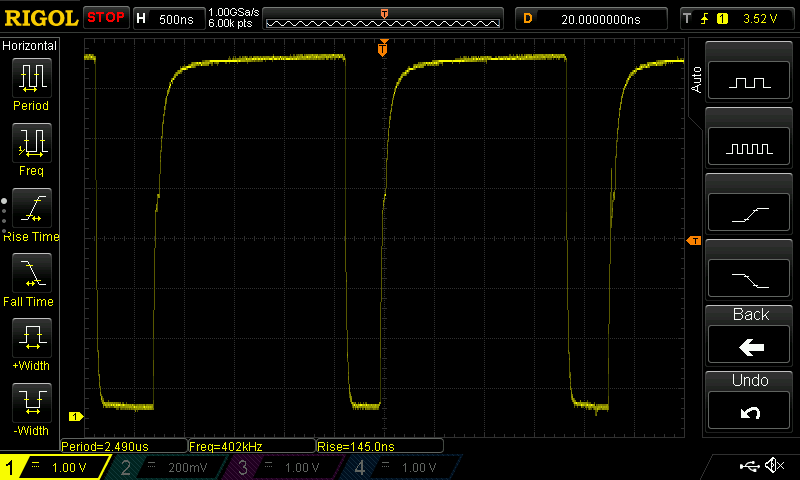
\includegraphics[width=1\textwidth]{duty_130.png}
    \caption{Wypełnienie sygnału sterującego przy napieciu wyjściowym 130 V}
    \label{fig:duty_130}
\end{figure}

\begin{figure}[H]
    \centering
    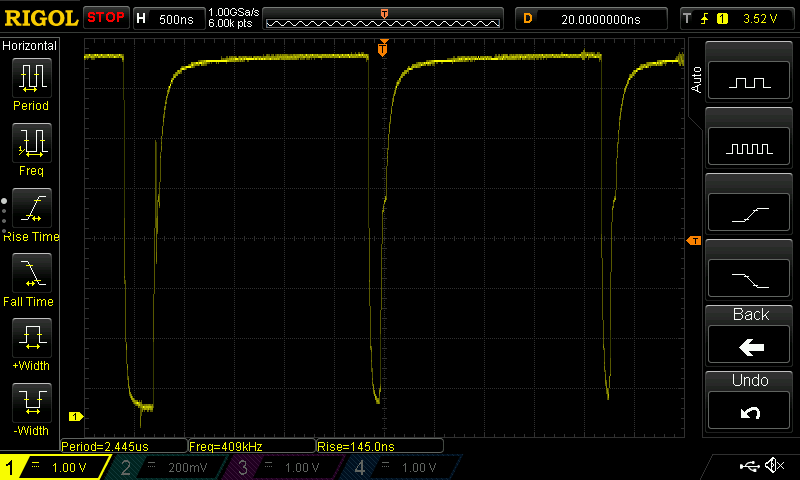
\includegraphics[width=1\textwidth]{duty_210.png}
    \caption{Wypełnienie sygnału sterującego przy napieciu wyjściowym 210 V}
    \label{fig:duty_210}
\end{figure}

Jak widać na rysunku \ref{fig:duty_210}, przy wysokim wypełnieniu sygnału sterującego,
tranzystor nie do końca się zamyka, co powoduje, że napięcie wyjściowe jest mniejsze niż zakładane, 
a do tego tranzystor się nagrzewa i zwiększa się pobór mocy.

Może to wynikać ze źle dobranych elementów kompensujących w układzie przetwornicy.
Zmniejszony zakres w jakim można regulować napięcie wyjściowe nie wpłynie na działanie całego układu,
ponieważ górny limit napięcia wyjściowego przetwornicy nie jest krytyczny dla działania budzika.

\subsection{Testy poboru mocy}
Zaczęto od pomiarów mocy pobieranej przez cały układ. Pobór mocy układu zmierzono za pomocą zasilacza laboratoryjnego PS-305DF.
Zmierzono pobór mocy układu dla różnych napięć wyjściowych przetwornicy. Pobór mocy zawiera też w sobie pobór mocy pozostałych modułów,
ale jest on stały i niezależny od napięcia wyjściowego przetwornicy, więc sam kształt charakterystyki poboru mocy jest zależny od przetwornicy.
W podrozdziale \ref{sec:obliczenia_mocy} założono, że pobór mocy układu nie przekroczy 13 W, a sama przetwornica będzie pobierać około 6.5W.
Pomiary poboru mocy zamieszczono w tabeli \ref{tab:power}.

\begin{table}[H]
    \centering
    \begin{tabular}{|c|c|}
        \hline
        Napięcie wyjściowe [V] & Pobór mocy [W] \\
        \hline
        130 & 1.654 \\
        140 & 1.836 \\
        150 & 2.258 \\
        160 & 2.705 \\
        170 & 3.282 \\
        180 & 4.021 \\
        190 & 5.25 \\
        200 & 7.65 \\
        210 & 8.22 \\
        \hline
    \end{tabular}
    \caption{Zależność poboru mocy od napięcia wyjściowego}
    \label{tab:power}
\end{table}

Wykreślono zależność poboru mocy od napięcia wyjściowego na wykresie \ref{fig:power}.

\begin{figure}[H]
  \centering
  \begin{tikzpicture}
    \begin{axis}[
      xlabel={Napięcie wyjściowe [V]},
      ylabel={Pobór mocy [W]},
      legend pos=north west,
      grid=major,
      width=0.8\textwidth,
      height=0.4\textwidth,
      ]
      \addplot[color=blue] coordinates {
        (130, 1.654)
        (140, 1.836)
        (150, 2.258)
        (160, 2.705)
        (170, 3.282)
        (180, 4.021)
        (190, 5.25)
        (200, 7.65)
        (210, 8.22)
      };
    \end{axis}
  \end{tikzpicture}
  \caption{Wykres zależności poboru mocy od napięcia wyjściowego}
  \label{fig:power}
\end{figure}

Po dokonaniu pomiary poboru mocy, zaobserwowano, że pobór mocy jest większy niż zakładano i wynosi ponad 8 W przy napięciu wyjściowym 210 V.
Na charakterystyce pobór mocy okazał się nie liniowy przy wyższych napięciach wyjściowych. Wynika to ze spadku wydajności przetwornicy przy wyższych napięciach,
z powodu nie zamykania się tranzystora przełączającego. Jednak układ domyślnie ma procować na niższych napięcia, więc 
zdecydowano się na programowe ograniczenie napięcia wyjściowego przetwornicy do 190 V, gdzie układ pracuje z mocą zakładaną na etapie projektowania. Dolny limit napięcia wyjściowego również
został ograniczony do 140 V, ponieważ przy 130 V lampy nie zapalają się w pełni, co może prowadzić do ich uszkodzenia. 
Jako domyślne napięcie wyjściowe wybrano 150 V, przy którym pobór mocy wynosi 2.358 W, co jest akceptowalnym wynikiem.
Porównując ten pobór mocy z innymi zegarkami dostępnymi na rynku, jest on porównywalny.

Poza zmniejszonym zakresem pracy przetwornicy, wszystkie pozostałe założenia projektowe zostały spełnione. Układ 
pobiera czas z serwera czasu, wyświetla go na lampach nixie i działa jako budzik. Wszystkie funkcje działają poprawnie.

\end{document}


